\documentclass{article}

% Use utf-8 encoding for foreign characters
\usepackage[utf8]{inputenc}

% Setup for fullpage use
\usepackage{fullpage}
\usepackage{graphicx}
\usepackage{hyperref}
\usepackage[french]{babel}
\usepackage[final]{pdfpages}
\usepackage{times}
\usepackage{gensymb}
\usepackage{color}
\usepackage{array}
\usepackage{textcomp}
\usepackage{subfig}
\usepackage{amsmath}
\usepackage{titlesec}
\usepackage{tabularx}
\includepdfset{pages = -, pagecommand = {}, scale = 0.9}
\setcounter{secnumdepth}{4}
\newcommand{\placeholder}[1]{{\noindent \color{red}[ #1 ]}}
\newtheorem{Rem}{Remarque}
\titleformat{\paragraph}
{\normalfont\normalsize\bfseries}{\theparagraph}{1em}{}
\titlespacing*{\paragraph}
{0pt}{3.25ex plus 1ex minus .2ex}{1.5ex plus .2ex}



\begin{document}
\section{Groupement des Régions}
	Avant de pouvoir classer les différentes régions/provinces en groupes, nous devons effectuer les calculs pour obtenir la matrice des distances.
	
	La voici:
	
\begin{tabularx}{18.4cm}{|X|X|X|X|X|X|X|X|X|X|X|}
	\hline
	X/Y                      &Bruxelles / Brussels&Antwerpen &Limburg (BE) &Oost-Vlaanderen &Vlaams-Brabant &West-Vlaanderen &Brabant Wallon &Hainaut &Liège &Luxembourg (BE)\\
	\hline
	Antwerpen                           &2.1976387 &&&&&&&&&\\                                                                                                                             
	\hline
	Limburg (BE)                        &3.7924177       &1.6421791&&&&&&&&\\                                                                                                                                                         
	\hline
	Oost-Vlaanderen                     &1.8915634       &0.4301455          &1.9210062&&&&&&&\\                                                                                                                                      
	\hline
	Vlaams-Brabant                      &0.4977661       &2.4667642          &4.0669507             &2.1495597&&&&&&\\                                                                                                                
	\hline
	West-Vlaanderen                     &3.8006950       &1.6560244          &0.1286935             &1.9409271            &4.0820783 &&&&&\\                                                                                           
	\hline
	Brabant Wallon                      &1.9575174       &3.9798765          &5.5491930            & 3.6703024            &1.7755390             &5.5680656                                                                     &&&&\\
	\hline
	Hainaut                             &3.7125903       &1.5599647          &0.1778578            & 1.8341168            &3.9730810             &0.2564549            &5.4790390                                                &&&\\
	\hline
	Liège                               &2.8325198       &0.7078850          &0.9826074            & 0.9572507            &3.0928177             &1.0089326            &4.6193113     &0.8853731                                  &&\\
	\hline
	Luxembourg (BE)                     &4.7062104       &2.5412458          &0.9393496             &2.8423194            &4.9768604             &0.9233110            &6.4807544     &1.0232601   &1.8917065                      &\\
	\hline
	Namur                         &3.5118824       &1.4269053          &0.5102366             &1.6929400            &3.7991224             &0.5027041            &5.3359194     &0.4713670   &0.7868244             &1.2514964\\
	\hline
\end{tabularx}
	
	Après avoir calculé ces distances, nous devions pouvoir trouver un moyen de regrouper ces distances pour pouvoir à la fin les classer en différents groupes. Pour cela, nous avons réalisé l'arbre des distances qui contient, sous forme d'arbre les relations entre chaque composante en fonction de sa distance par rapport aux autres. Le résultat est obtenu via l'algorithme suivant:
	
	\begin{itemize}
		\item[Etape 1] n élément à classer
		\item[Etape 2] Calculer la matrice des distances et chercher les individus pour lesquels la distance est minimale. 
		Agréger ces éléments en un seul élément (ils seront frères dans l'arbre). On obtient à la fin une partition à n-1 éléments.
		\item[Etape 3] On recrée la matrice des distances avec ces modifications apportées et on boucle sur la 2$^{\text{ème}}$ étape jusqu'à ce que tous les individus soient contenus dans une seule classe (la racine de l'arbre).
	\end{itemize}
	
	A l'aide de cet algorithme nous avons obtenu cet arbre:
	
		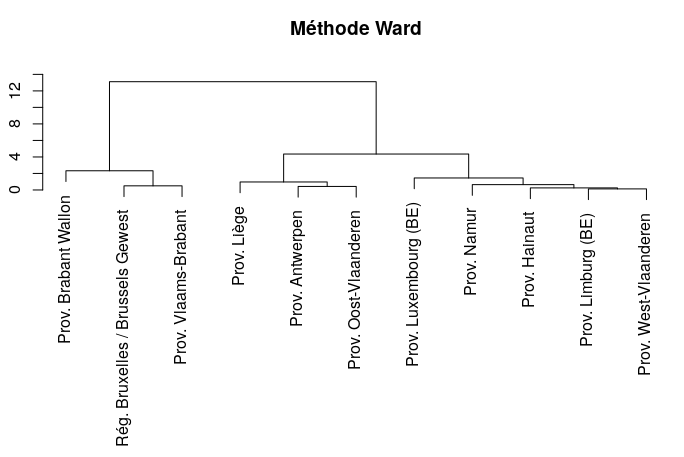
\includegraphics[width=12cm,height=7cm]{tree}
	
	Pour réaliser celui-ci nous avons appliqué le critère de Ward généralisé qui dit que l'on doit rechercher les éléments pour lesquels la perte d'inertie interclasse est minimale.
	
	\frame{$\Delta I_{ii'} = \frac{m_im_{i'}}{m_i + m_{i'}}d^2(x_i,x_{i'}$}
	
	Maintenant que nous avons notre arbre des distances nous pouvons nous atteler à la tâche de diviser celui-ci en différentes classes. Comment faire cela ? Nous devons nous intéresser à la décroissance de l'inertie intraclasse. En effet, lorsque celle-ci diminue de manière plus faible cela veut dire que le nombre de groupe choisi est optimal.
	
	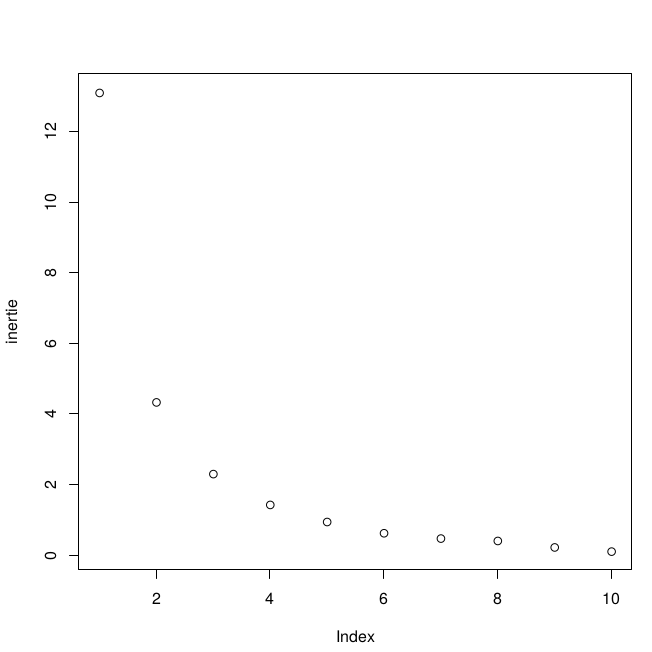
\includegraphics[width=\textwidth]{Inertie}
	\newpage
	D'après ce graphique, on pourrait classer nos individus en 5 groupes puisque c'est à ce niveau que l'inertie intraclasse se stabilise $\Rightarrow$ le critère d'optimalité.
	
	Avec toutes ces données nous pouvons donner une forme finale à notre arbre des distances qui contiendra les différents groupes d'individus.
	
	Le voici : 
	
	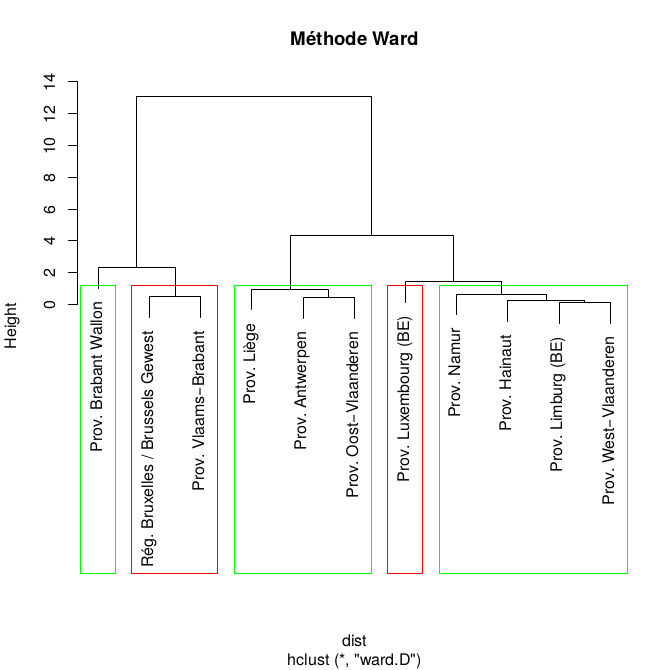
\includegraphics[width=\textwidth]{Ward}
	
	Ce graphique nous montre la classification de nos régions qui ont les mêmes comportements au fur et à mesure du temps.
\end{document}